\section{Transporting the parameterization to another collision energy}
\label{sec:energy_transport}

\textcolor{red}{DRAFT --- the $13$~TeV validation below is complete, and the $14$~TeV one
rests on the three samples generated so far; both sets of numbers are real, and the
sample counts behind them are stated wherever they matter. The $100$~TeV statements are a
placeholder and are marked where they appear.}

The $A$-coefficients of this report are extracted independently at each collision energy,
from a grid of samples generated at that energy. That is the reason the $13$, $13.6$ and
$100$~TeV results exist and $14$~TeV does not: the cost of the method is one full grid per
energy. This section asks whether a grid at one energy can be transported to another, so
that a new energy costs parton densities rather than simulation.

The observation it rests on is that a change of collision energy acts on the initial state
only. For a given partonic configuration the matrix element --- and with it the entire
dependence on the Wilson coefficients --- is unchanged; what changes is the luminosity with
which that configuration is produced, and parton densities give it.

Concretely, the partonic invariant mass is $\hat{s} = x_1 x_2 s$. Holding $\hat{s}$ fixed
while the collider energy changes from $\sqrt{s}$ to $\sqrt{s}'$ requires the momentum
fractions to move as $x_i \to x_i \sqrt{s/s'}$, which also leaves the rapidity
$y = \tfrac{1}{2}\ln(x_1/x_2)$ unchanged. With $\hat{s}$ and $y$ both fixed the entire
final state is untouched: each event keeps its own \mHH, and only its weight changes.
Since $\mathrm{d}\sigma/\mathrm{d}\hat{s}\,\mathrm{d}y = s^{-1}\sum_{ab} f_a f_b
\hat{\sigma}_{ab}(\hat{s})$, that weight is
%
\begin{equation}
w = \frac{s}{s'}\,
    \frac{f_a(x_1',\mu)\,f_b(x_2',\mu)}{f_a(x_1,\mu)\,f_b(x_2,\mu)},
\qquad \mu = \mHH/2 ,
\label{eq:energy_kernel}
\end{equation}
%
evaluated event by event with that event's own incoming flavours $a,b$ and momentum
fractions, taken from the generator record. Only $90.2\%$ of these events are initiated by two gluons, so a gluon-only kernel
would approximate a tenth of the rate. The factorization scale is the same $\mHH/2$ used in the
generation, and the parton densities are the \textsc{PDF4LHC21\_40} set the samples were
produced with.

Histogramming the reweighted events gives one factor $K^j$ per bin. Because the
$A$-coefficients are linear in the yields and $K^j$ multiplies every yield in bin $j$
alike, the transport commutes with the extraction:
$A^j_k(\sqrt{s}') = K^j A^j_k(\sqrt{s})$ for all forty coefficients $k$. The published
determination at one energy can therefore be rescaled into one at another without
refitting anything.

Little else changes. The \emph{basis} is untouched. Its 40 points are positions in coupling
space, chosen in Sec.~\ref{sec:basisopt} to control how the simulation statistics of the
basis samples propagate into a prediction, and that criterion involves the monomials and
the samples' uncertainties but not the beam energy. The morphing weights $w_i(c)$ that
the matrix method solves for are likewise functions of the couplings alone
(Eq.~\eqref{eq:matrixmethod}), so they are identical at $13$, $13.6$ and $14$~TeV. What
changes between those energies is only the \emph{content} of each template, bin by bin,
and that is what $K^j$ supplies.

An analysis moving between LHC energies therefore keeps the same 40 points, the same
morphing and the same code, and swaps one coefficient file for another. This does not
extend to a collider of very different energy, where the accessible \mHH range itself
changes and the basis has to be reconsidered; that case is taken up in
Sec.~\ref{sec:energy_beyond}.

The \emph{prediction} is built from the $13.6$~TeV samples and parton densities, and from
nothing else: no sample at the target energy enters it, which is why $14$~TeV is reachable
at all. The \emph{validation} compares that prediction with samples generated at the target
energy which took no part in building it. Those samples appear on one side of the
comparison only and are never used to fit coefficients. The one quantity the method cannot
predict is the overall normalization of the transport, so the shape is quoted with a single
constant removed.

\paragraph{How many points the validation needs.}
The factorization argument says the kernel acts on the initial state, and therefore that
it is the same at every point of the nine-dimensional coupling space. That is a testable
statement rather than an assumption, and the reweighting samples of
Sec.~\ref{sec:grids} already exist at both $13$ and $13.6$~TeV, so it is tested on all of
them: the per-point rate closures scatter by $0.268\%$ against a mean statistical
uncertainty of $0.678\%$, a pull RMS of $0.30$. The points agree with one another more
closely than their own simulation statistics, so no coupling dependence of the energy
factor is resolved.

That is what makes a small validation set sufficient. Once the kernel is known not to
depend on the couplings, each additional point buys statistical precision and nothing
else, so the question is how much precision the comparison needs. Subsampling the $13$~TeV
closure answers it: the pull width is unbiased at every set size, $0.99$ to $1.00$ from
three points upwards, while the uncertainty on that width falls from $\pm 1.29$ at three
points to $\pm 0.059$ at ten and $\pm 0.040$ at twenty. Ten points resolve an excess
spread of about $0.35$ times the simulation uncertainty, roughly $1.4\%$ per bin, which
is below the modelling uncertainty of Sec.~\ref{sec:uncertainties}; beyond that the
validation is limited by what it is being compared against rather than by its own size.
The results below accordingly use a set of ten points at $13$~TeV, chosen greedily on
\mHH shape distance from the matrix-method basis and spanning the parameterization with a
maximum pairwise cosine of $0.957$ in monomial space, and the three points available so
far at $14$~TeV.

\paragraph{The kernel.}
The left panel of Fig.~\ref{fig:energy_transport} shows what the transport corrects and
what it leaves. It is built from ten validation points at $13$~TeV and the three
generated so far at $14$~TeV, which is why the $14$~TeV series is binned more coarsely;
the shaded region on its unchanged curve is the corresponding uncertainty.
Applied unchanged, the $13.6$~TeV coefficients are wrong by $+9\%$ at threshold rising to
$+21\%$ in the tail at $13$~TeV, and by $-5\%$ falling to $-13\%$ at $14$~TeV: the two
curves fall on opposite sides of unity because the source energy lies between the two
targets, and the error grows with \mHH because producing a given \mHH at a lower beam
energy requires larger momentum fractions, where the parton densities fall steeply.
Transported with Eq.~\eqref{eq:energy_kernel}, both agree with the generated samples to
better than $3\%$ over $250$~GeV to $2$~TeV, and to better than $1\%$ below $900$~GeV
where the samples are large enough for the comparison to be sharp. The residual scatter
is of the size of the statistical uncertainty of the generated samples themselves, which
the error bars show; no trend with \mHH survives the transport.

\paragraph{The coefficients, in three dimensions.}
The kernel test above is performed on \mHH spectra. What an analysis deploys is the
coefficient file, and there the kernel is applied per cell of
$(\pt^{HH}, |\cos\theta^*|, \mHH)$ rather than per \mHH bin. A per-cell error that is too
large at low \pt and too small at high would cancel in the projection onto \mHH and leave
the spectrum test unchanged, so the two are not equivalent and the second does not follow
from the first.

The transported file is therefore closed cell by cell: the polynomial it carries is
evaluated at the couplings of every validation sample and compared with what was generated
there, in each of the $9 \times 4 \times 40$ cells of the fit. Above $1$~TeV the
parameterization is one-dimensional --- the 36 $\pt$--$|\cos\theta^*|$ cells of a given \mHH
bin carry identical values --- so the cell rule takes one cell there and sums them below,
a factor 36 that was verified explicitly rather than assumed.

The right panel of Fig.~\ref{fig:energy_coeff_pulls} expresses the outcome as a pull:
the residual of each cell divided by its own simulation uncertainty. Only the region
below $1$~TeV enters it, where the fit is genuinely three-dimensional. If the coefficients are correct and the
only scatter is the finite number of simulated events, this distribution is a unit Gaussian
by construction, and anything the transport breaks appears as excess width.

The comparison is made on the basis points themselves, which is where the transported file
is actually used: the matrix method builds every other prediction out of those forty
templates, so if the transport is right there it is right everywhere the method is
defined. The measured widths are $0.981$ for the untransported $13.6$~TeV determination,
where all forty basis points were generated, $1.001$ transported to $13$~TeV, where
thirty-five of the forty exist, and $0.989$ transported to $14$~TeV, where three do. The
untransported determination is the floor of the comparison --- the transport cannot be
more accurate than what it transports --- and the two transported files are
indistinguishable from it. The $14$~TeV histogram is visibly the coarsest of the three
for the same reason: it is three samples against forty.

Two caveats belong with that statement. The first is a residual median pull of $-0.034$ at
$13.6$~TeV, reproduced at $-0.035$ after transport to $13$~TeV: a bias of a few percent of
the simulation uncertainty that is present in the source and is therefore a property of
the determination, not of the transport. The second is the $490$--$510$~GeV bin of the
delivered $13.6$~TeV fit, which closes at $0.6446 \pm 0.0005$ against its own samples
while its neighbours close at unity; it is excluded from the figure and from the widths
above. \textcolor{red}{Matheus: this bin looks like a defect of the delivered
$13.6$~TeV fit rather than anything to do with the transport, and is worth a look.}
At $14$~TeV the three available samples make the width itself uncertain by $\pm 1.3$, so
the agreement seen there confirms the implementation rather than measuring the accuracy of
the transport; the remaining thirty-seven basis points are in production, which will close
that energy on the complete basis as well and bring the uncertainty to about $\pm 0.03$.

\begin{figure}[htbp]
\centering
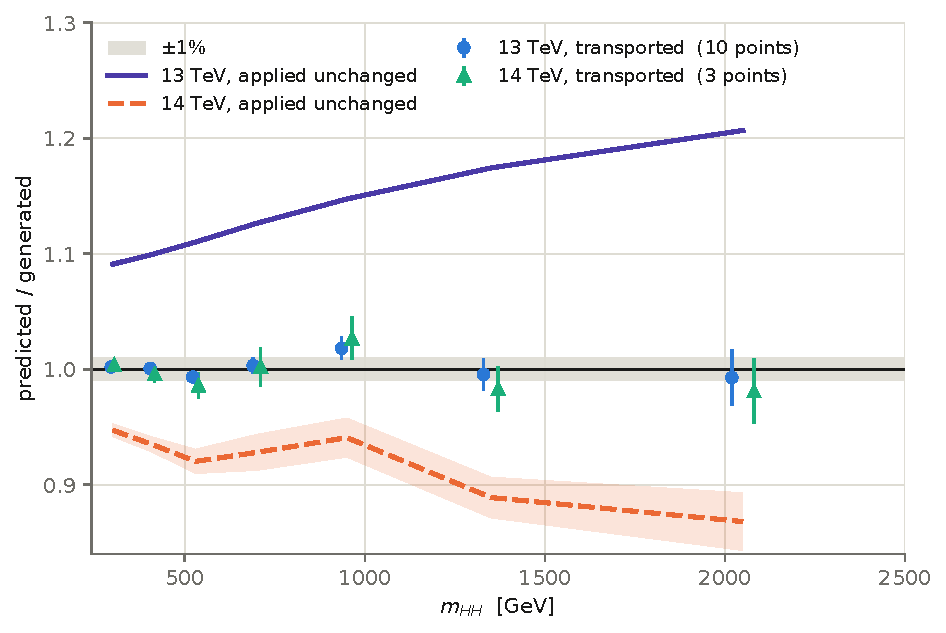
\includegraphics[width=0.49\linewidth]{plots/energy_transport_13TeV.pdf}
\hfill
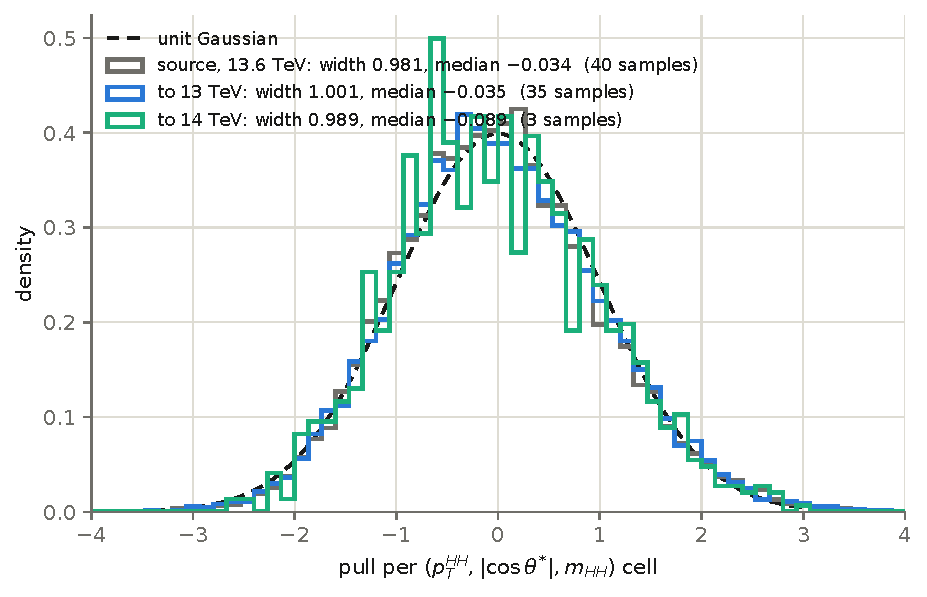
\includegraphics[width=0.49\linewidth]{plots/energy_coeff_pulls_3d.pdf}
\caption{Left: ratio of predicted to generated \mHH spectrum at $13$ and $14$~TeV, with
the $13.6$~TeV parameterization applied unchanged (lines) and transported with
Eq.~\eqref{eq:energy_kernel} (points, overall constant removed); the band marks
$\pm 1\%$. Right: pull of the transported $A$-coefficients per
$(\pt^{HH}, |\cos\theta^*|, \mHH)$ cell, on the basis points, against a unit Gaussian
(dashed). Both are described in the text.}
\label{fig:energy_transport}
\label{fig:energy_coeff_pulls}
\end{figure}

\textcolor{red}{Matheus: the complete forty-point basis is being generated at every
energy --- five points are missing at $13$~TeV and thirty-seven at $14$~TeV, the former a
subset of the latter, so it is one request. With those in hand the right panel closes on
the full basis at all three energies, with no caveat about which subset was available,
and the $14$~TeV pull width goes from an uncertainty of $\pm 1.3$, which says nothing, to
about $\pm 0.03$.}

\paragraph{Two further checks.}
The kernel of Eq.~\eqref{eq:energy_kernel} is exactly invertible, so running the machinery
in the opposite direction --- transporting the $13$~TeV samples up to $13.6$~TeV --- must
return the inverse constant. It does, $1.0098$ against $1/0.9902 = 1.0099$, which is a
check on the implementation and not on the physics.

The second check is the configuration an analysis actually deploys. Only the forty basis
templates are transported; every other coupling point is then built from them by the
matrix method, whose weights are the same at every energy. Closing the morphed prediction
against the reweighting samples of Sec.~\ref{sec:grids} leaves the agreement unchanged in
the bulk, and in the tail the comparison becomes limited by the statistics of the basis
samples themselves, amplified by the morphing weights: the matrix method's own statistical
uncertainty on the morphed prediction is $8\%$ per bin below $1$~TeV and $38\%$ above it,
and every per-bin deviation lies within $0.6$ of that uncertainty, with a mean pull of
zero. The transport introduces no bias that the available statistics can detect; what
limits the tail is the size of the basis samples, not the transport.

\paragraph{The covariance.}
The coefficients are delivered with their covariance, and it has to be transported
too. Because the kernel multiplies all forty coefficients of a cell by the same
number, the covariance of that cell transforms quadratically rather than linearly:
%
\begin{equation}
C_{kl}(\sqrt{s}',j) = K_j^2 \left[ C_{kl}(\sqrt{s},j)
                      + r_j^2\, A_k^j A_l^j \right] ,
\label{eq:energy_cov}
\end{equation}
%
where $r_j$ is the relative statistical uncertainty of $K_j$. The factor $K^2$ is the
part that is easy to get wrong: reusing the $13.6$~TeV covariance unchanged would
leave the uncertainties $30\%$ too large at $13$~TeV and $8\%$ too small at $14$, in
opposite directions.

The second term is the uncertainty of the kernel itself. It is rank one and fully
correlated across the forty coefficients of a cell, so it does not average down
within a cell, and it is not negligible: $r$ has a median of $1.8\%$ per cell, while
a quarter of the $57600$ coefficient entries carry a relative uncertainty smaller than
that. Where the one-dimensional region or a noisy cell makes the transport fall back on
the \mHH-projected kernel, $r$ is the projected kernel's own uncertainty, $0.3\%$,
since that is measured on all $36$ $\pt$--$|\cos\theta^*|$ cells together.

Two uncertainties are deliberately left outside Eq.~\eqref{eq:energy_cov} because a
per-cell matrix cannot express them. The parton-density uncertainty on $K$ is
correlated between bins, and the overall normalization of the transport is a single
number correlated across every bin and coefficient; both are carried as nuisance
parameters alongside.

\subsection{Beyond the LHC}
\label{sec:energy_beyond}

\textcolor{red}{PLACEHOLDER. The transport is not used for the $100$~TeV results.
Reweighting redistributes the events that exist; it cannot create an event at a partonic $\hat{s}$ the source sample
never produced. The $13.6$~TeV samples place $7.5\times 10^{-5}$ of their rate above
$3$~TeV and the highest bin holding more than a thousand effective events is
$3.75$~TeV, so a transported $100$~TeV prediction would be blind in exactly the region
that motivates such a collider. The kernel is also no longer gentle --- median $30$,
spanning $5$ to $270$, with weights reaching $3800$ --- and it costs between a half and
two thirds of the effective sample size. The $100$~TeV coefficients are therefore
extracted from $100$~TeV simulation in the usual way, and the basis is re-optimized
there rather than inherited.}
